\documentclass[12pt,a4paper]{article}
\usepackage[utf8]{inputenc}
\usepackage{amsmath}
\usepackage{amsfonts}
\usepackage{amssymb}
\usepackage{lmodern}
\usepackage{graphicx}
\usepackage{geometry}
\usepackage{listings}
\usepackage{color}
\usepackage[linesnumbered,ruled,vlined]{algorithm2e}

\setlength{\parindent}{0em} 

\newcommand\mycommfont[1]{\footnotesize\ttfamily\textcolor{blue}{#1}}
\SetCommentSty{mycommfont}

\geometry{
	a4paper, 
	top=25mm, 
	left=25mm, 
	right=25mm, 
	bottom=30mm,
	headsep=10mm, % Abstand zwischen Kopfzeile und Text
	footskip=12mm 
}

\lstdefinestyle{java}{
  language=Java,
  frame=none,
  aboveskip=3mm,
  belowskip=3mm,
  showstringspaces=false,
  columns=flexible,
  basicstyle={\small\ttfamily},
  numbers=none,
  keywordstyle=\color{blue},
  commentstyle=\color{green},
  stringstyle=\color{cyan},
  breakatwhitespace=true,   
  captionpos=b,    
  breaklines=true,                                   
  tabsize=2
}
\lstset{style=java}

\title{Report: File Transfer}
\author{Wu, Wei, 2012220748 \\ Kölker, Stephan, 2015403217}
\begin{document}

\maketitle

\section{Source Code and Algorithms}

\subsection{Language and Libraries}
We implemented the file transfer program by using Java without any external libraries. The socket connection was built using the \lstinline!java.net! package.

\subsection{Program Architecture}
The core classes of our program consists of four different classes: \lstinline!FileTransferClient! and \lstinline!FileReceiveHandler! on the client side and \lstinline!FileTransferServer! and \lstinline!FileSendHandler! on the server side. \lstinline!FileTransferClient! and \lstinline!FileTransferServer! create the socket connection, a thread pool with multiple threads (number of system cores) and hand the threads as well as the file to be transferred to the executing thread.

To transfer a file, we use \lstinline!FileSendHandler! and \lstinline!FileReceiveHandler!. They implement both the interface \lstinline!Runnable!, so they can be executed in a thread. We first transfer the full file path, then the size of the file to the sender. After that, the actual file content follows. Several chunks (size: about 10KB) will be read and sent iteratively since the system probably cannot hold the whole file into memory at once. On the receiver's side, we also read the file in the same chunks and write them to file. 

For each file we use a single TCP connection to achieve the highest possible concurrency. But as the number of threads increases, we will end up with a bottleneck because of the thousands of tiny files. To avoid a bottleneck in computing power and bandwidth, we create a zip folder of the folder ``thousands\_of\_tiny\_files'' and transfer this via an own TCP connection. On the other side, the zip folder is unzipped and the actual files are stored to the hard disk.

Besides the above-mentioned classes, we use some helper classes: \lstinline!Config! to read from the configuration file, \lstinline!DirectoryManager! to create directory paths recursively or \lstinline!ZipUtil! that we use to ``zip'' a directory.

The main class is \lstinline!Main!. Starting the program takes one parameter: ``server'' or ``client''. All settings are defined in \lstinline!config.properties! in the \lstinline!resources! folder.

\subsection{Program Sequence}
The following sequence diagram illustrates the optimal program flow without any errors. In the development of this application, we focused on the file transmission and transmission possibilities to enhance the throughput. So, we mostly ignored error handling. In case of errors, the application will directly throw java exceptions. 

\begin{figure}[h!]
	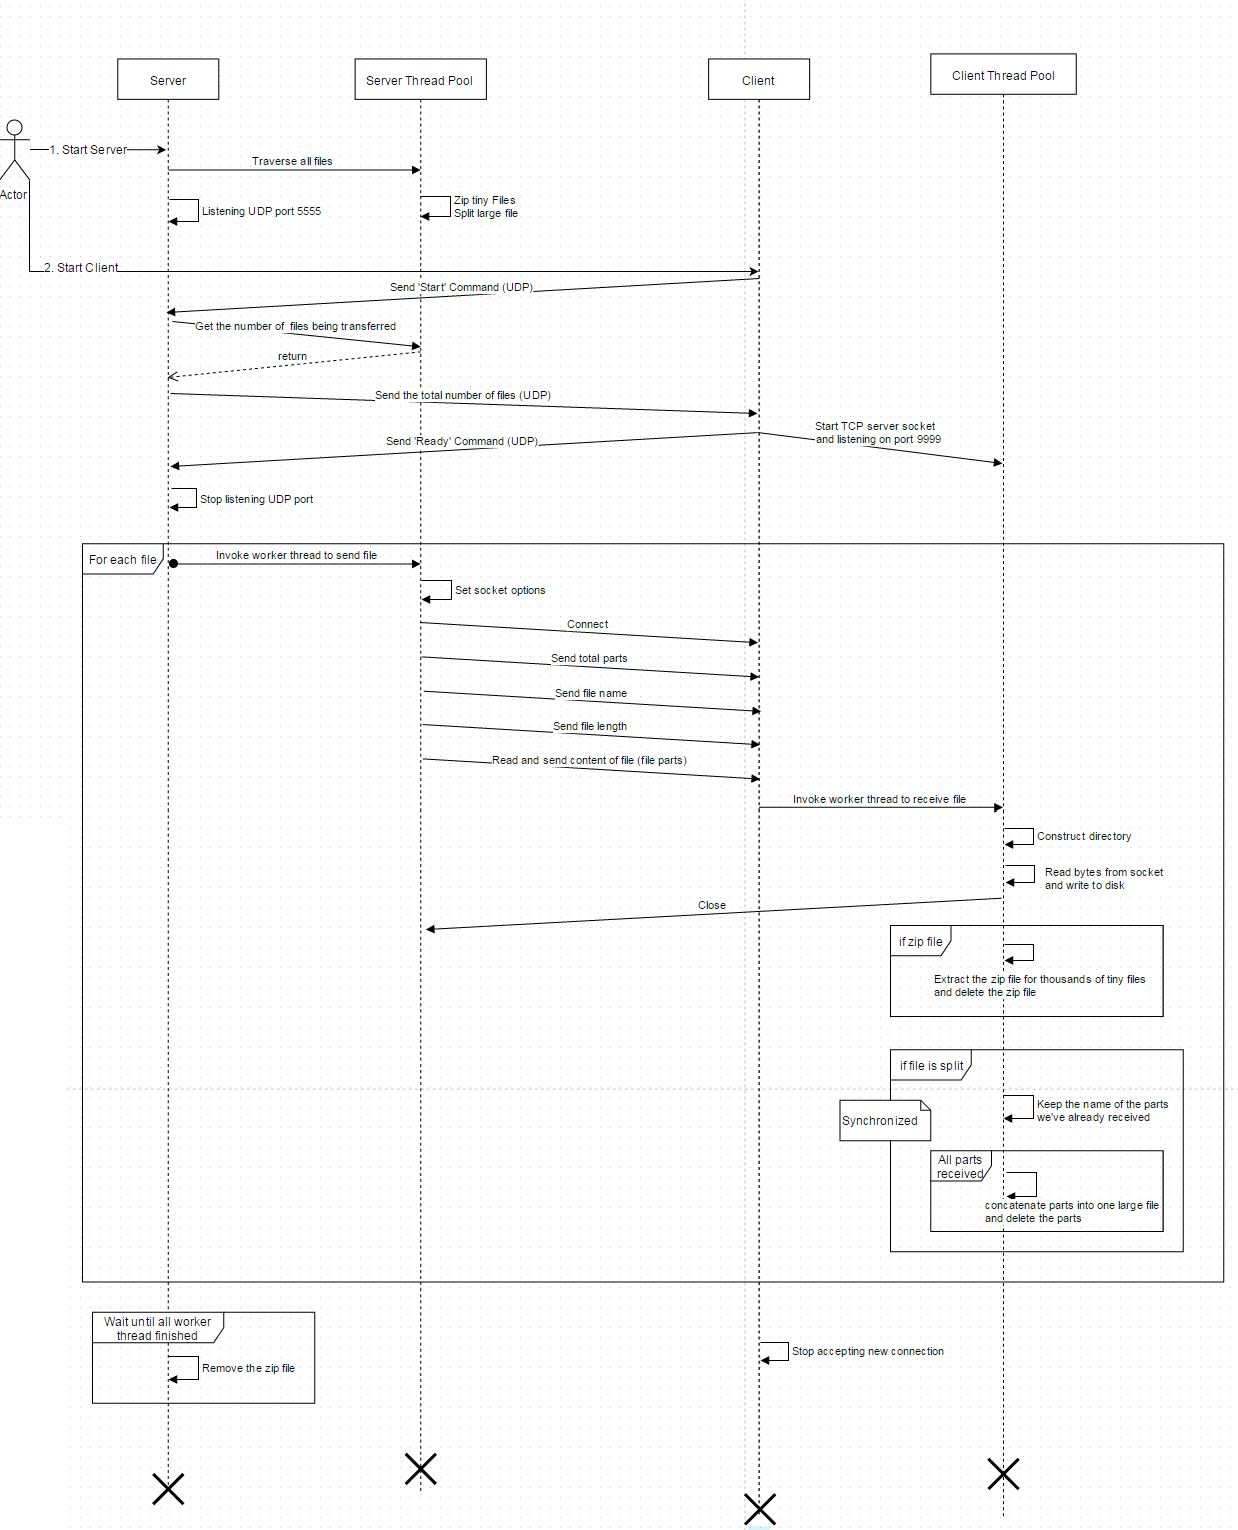
\includegraphics[scale=.5]{./FileTransferApp.png}
	\caption{Program flow without errors}
\end{figure}

\subsection{Alternatives and Decisions}
During the development process, we tested various alternative classes whether they perform better than the above-mentioned classes.

The very first decision was: C++ or Java? Although C++ is known to be much faster and more efficient than Java, it also depends on the programmer and on the optimization possibilities. We are convinced that C++ does not offer much optimization possibilities in this small application and hence, the run-time of the programs in both languages should be more or less equal. We also decided for Java because one of us was not very familiar with programming in C++.

As an alternative to the \lstinline!java.net! socket classes, the channel classes in the \lstinline!java.nio.channels! package provide a more low-level approach in Java to perform IO operations. It provides various file- and socket-related classes. But in some speed tests, we could not determine any time difference between both method and hence, we decided for the classical IO classes.

The transmission of the biggest file consumes the most transmission time. To avoid this bottleneck, it would be useful to split this file into several parts (e.g. 4 parts) and transfer them independently. The problem in this alternative is the file reconstruction at the receiver's side. When using the same file name, we can determine which parts belong together and with an additional byte that determines their order, even ordering would not be a problem. But we writing concurrently from several threads into one file is much more complicated: Since every file part has its own offset and length, we must leave this offset free in the file. Current file systems do not support leaving $x$ bytes free and then write $y$ bytes. A possible solution would be first to write $x$ zeros and then $y$ bytes. This is very ineffective. Another solution is to store all parts whose predecessor is not completely arrived yet in the memory and write them to disk as soon as their predecessor was written to disk. But this maybe could cause memory overflows. If for example the first file part arrives at last, the whole file has to be stored in the memory. This is the reason why we did not implemented it.

Another try was to implement UDP-based transmission for the small files. Since UDP transmissions have less overhead than TCP, the transmission would be much faster and in the test system, we have a closed world without any collisions and a very small transfer line. Nevertheless, the correctness of the transferred data is important and using UDP without ensuring the correctness is nothing but a game of luck. Of course, one could simply use a hash method as a checksum of every message make sure, the data is correct. But we decided against this approach, because even with a checksum the data could still be false.

\section{TCP Enhancements}
We set the buffer size of both, sender and receiver, to 64KBytes. Moreover, we turn of Nagle's algorithm to make sure, the data is immediately sent after flushing it. We also set SO linger to an interval of 60.

Furthermore, we tried to enhance the network's MTU, but did not found a way to manipulate this using Java (except by calling a bash script).

\end{document}